In this section, we introduce quantum gates and demonstrate their use in \MindQuantum. We categorize quantum gates into three types: fixed quantum gates, parameterized quantum gates, and custom quantum gates. Additionally, we utilize the \code{on()} method to set target and control qubits and the \code{controlled()} function for adding control qubits to multiple gates.

\subsubsection{Quantum Gates Overview}

In quantum computing, quantum gates are fundamental operations that manipulate qubits, the basic units of quantum information. Analogous to classical logic gates that operate on bits, quantum gates act on qubits and are represented mathematically by unitary matrices, preserving the quantum state's normalization and reversibility.

Quantum gates are essential for constructing quantum circuits and implementing quantum algorithms by performing operations such as rotations, flips, and entanglement creation. These operations enable unique computational capabilities distinct to quantum computers.

Quantum gates are categorized based on the number of qubits they act upon: single-qubit gates modify individual qubit states, while multi-qubit gates facilitate interactions between qubits, enabling complex quantum operations and entanglement. Gates can also be classified as non-parameterized (e.g., \X, \Y, \Z, \H) or parameterized (e.g., \RX, \RY, \RZ), the latter providing additional computational flexibility. In \MindQuantum, these gates---including parameterized ones using \ParameterResolver---are easily constructed.

\subsubsection{Fixed Quantum Gates}
Fixed quantum gates perform specific operations on quantum states, represented by unitary matrices. Here are some examples for a qubit state $\ket{\phi}=a\ket{0}+b\ket{1}$:

\begin{align*}
    I\ket{\phi} & =
    \begin{bmatrix}
        1 &  & 0 \\
        0 &  & 1
    \end{bmatrix}
    \begin{bmatrix}
        a \\
        b
    \end{bmatrix}=
    \begin{bmatrix}
        a \\
        b
    \end{bmatrix},  \\
    X\ket{\phi} & =
    \begin{bmatrix}
        0 &  & 1 \\
        1 &  & 0
    \end{bmatrix}
    \begin{bmatrix}
        a \\
        b
    \end{bmatrix}=
    \begin{bmatrix}
        b \\
        a
    \end{bmatrix},  \\
    Y\ket{\phi} & =
    \begin{bmatrix}
        0 & -i \\
        i & 0
    \end{bmatrix}
    \begin{bmatrix}
        a \\
        b
    \end{bmatrix}=
    \begin{bmatrix}
        -bi \\
        ai
    \end{bmatrix},  \\
    Z\ket{\phi} & =
    \begin{bmatrix}
        1 & 0 \\
        0 & -1
    \end{bmatrix}
    \begin{bmatrix}
        a \\
        b
    \end{bmatrix}=
    \begin{bmatrix}
        a \\
        -b
    \end{bmatrix}, \\
    H\ket{\phi} & =
    \frac{1}{\sqrt{2}}
    \begin{bmatrix}
        1 & 1  \\
        1 & -1
    \end{bmatrix}
    \begin{bmatrix}
        a \\
        b
    \end{bmatrix}=
    \frac{1}{\sqrt{2}}
    \begin{bmatrix}
        a+b \\
        a-b
    \end{bmatrix}.
\end{align*}

Example usage in \MindQuantum:
\begin{lstlisting}
from mindquantum.core.gates import H, SWAP

h = H.on(0)
swap = SWAP.on([0, 1])
print(swap)
\end{lstlisting}
The output is:
\begin{lstlisting}
SWAP(0 1)
\end{lstlisting}

\subsubsection{Parameterized Quantum Gate}
Pauli matrices are very important matrices, and they form a set of bases for spatial operators. When the Pauli matrix appears on the exponents, three classes of useful unitary operators are produced, namely rotation operators with respect to $\hat{x}, \hat{y}, \hat{z}$, defined by the following equations.

\begin{align*}
    Rx(\theta) & =
    e^{-\frac{i\theta X}{2}}=
    \cos{\frac{\theta}{2}}I-i\sin{\frac{\theta}{2}}X \\
               & =\begin{bmatrix}
        \cos{\frac{\theta}{2}}   &  & -i\sin{\frac{\theta}{2}} \\
        -i\sin{\frac{\theta}{2}} &  & \cos{\frac{\theta}{2}}
    \end{bmatrix},        \\
    Ry(\theta) & =
    e^{-\frac{i\theta Y}{2}}=
    \cos{\frac{\theta}{2}}I-i\sin{\frac{\theta}{2}}Y \\
               & =    \begin{bmatrix}
        \cos{\frac{\theta}{2}} &  & -\sin{\frac{\theta}{2}} \\
        \sin{\frac{\theta}{2}} &  & \cos{\frac{\theta}{2}}
    \end{bmatrix},    \\
    Rz(\theta) & =
    e^{-\frac{i\theta Z}{2}}=
    \cos{\frac{\theta}{2}}I-i\sin{\frac{\theta}{2}}Z \\
               & =    \begin{bmatrix}
        e^{\frac{-i\theta}{2}} &  & 0                     \\
        0                      &  & e^{\frac{i\theta}{2}}
    \end{bmatrix}.
\end{align*}


Since there is an infinite number of $2*2$ matrices, the number of quantum gates is also infinite. According to the Z-Y decomposition, a unitary matrix $U$ over any single qubit can be represented as $U=e^{i\alpha}Rz(\beta)Ry(\gamma)Rz(\delta)$. Therefore, in order to construct general quantum gates, it is necessary to use parameters to construct rotating gates. There are three initialization methods provided in \MindQuantum, because \ParameterResolver has three initialization methods. Take the RX gate as an example:

\begin{lstlisting}
from mindquantum.core.gates import RX
from mindquantum.core.parameterresolver import ParameterResolver as PR
import numpy as np

rx1 = RX(0.5)
rx2 = RX('a')
rx3 = RX({'a': 0.2, 'b': 0.5})

a, b = PR('a'), PR('b')
rx4 = RX(0.2 * a + 0.5 * b)

mat_rx1 = rx1.matrix()
mat_rx4 = rx4.matrix(pr={'a': 1, 'b': 2})
\end{lstlisting}

Note that in the above demo, \code{rx1} is actually a non-parameterized gate, since we already set the rotation angle $\theta = 0.5$.

\subsubsection{Custom Quantum Gate}
Creating arbitrary quantum gates is sometimes necessary for specific applications. In \MindQuantum, two methods are available for constructing custom gates:

\textit{Universal Math Gate} -- If the matrix representation of a gate is known, it is convenient to construct the gate in \MindQuantum. Two parameters are required to initialize \UnivMathGate, which require the gate name and the matrix value. If the matrix is not unitary, the state vector cannot be normalized.
Example:
\begin{lstlisting}
from mindquantum.core.gates import UnivMathGate
import numpy as np

x_mat = np.array([[0,1],[1,0]])
custom_X_gate = UnivMathGate('custom_X', x_mat).on(0, 1)
print(custom_X_gate)
\end{lstlisting}

Output:
\begin{lstlisting}
custom_X(0 <-: 1)
\end{lstlisting}

\textit{Universal Parameterized Gate} -- For some applications we need to construct a parameterized gate in which the parameter is varying. In \MindQuantum, we can easily construct a customized parameterized gate by \geneunivparameterizedgate, and its usage is basically as same as that of \RX gate. Two parameters are required to initialize such a gate. One is a function or method to use only one parameter (similar to theta in \RX) to generate a unitary matrix, noting that no error is reported if the resulting matrix is not unitary. The other is the function or method that produces the derivative of this matrix, which is used to calculate the gradient. This method supports the generation of arbitrary qubit operators and can accelerate the performance by numba.JIT.

Example:
\begin{lstlisting}
from mindquantum.core.gates import gene_univ_parameterized_gate

def matrix(theta):
    return np.array([[np.exp(1j * theta), 0],
                     [0, np.exp(-1j * theta)]])

def diff_matrix(theta):
    return 1j * np.array([[np.exp(1j * theta), 0],
                          [0, -np.exp(-1j * theta)]])

TestGate = gene_univ_parameterized_gate('Test', matrix, diff_matrix)

# Non-parameterized usage
test1 = TestGate(0.5).on(0)

# Parameterized usage
test2 = TestGate('a').on(0)
\end{lstlisting}

\subsubsection{``On'' Method}
For some controlled quantum gates, we need to specify the target qubits and control qubits of the quantum gate. In \MindQuantum, we can implement this function through the \code{on()} method. This method takes two parameters. One is the target qubits and the other is the control qubits, both of which can be single qubit or multiple qubits. It is worth emphasizing that any gate can add arbitrary control operations.

Example:
\begin{lstlisting}
from mindquantum.core.gates import X

x = X.on(0, [1, 2])
print('Target qubit:{}, Control qubits:{}'.format(x.obj_qubits, x.ctrl_qubits))
\end{lstlisting}

Output:
\begin{lstlisting}
Target qubit:[0], Control qubits:[1, 2]
\end{lstlisting}

\subsubsection{``Controlled'' Function}
In addition to the \code{on()} method, we can also add control bits via the \code{controlled()} function. The \code{controlled()} function is used to add control qubits (which can be multiple) to any quantum circuit or quantum operator. For example, we build a quantum circuit containing only two qubits and add a control qubit q2 to it by \code{controlled()} method:
\begin{lstlisting}
from mindquantum.algorithm.library import qft
from mindquantum.core.circuit import controlled

u1 = qft(range(2))
u2 = controlled(u1)
u2 = u2(2)
u2.svg()
\end{lstlisting}

As shown in Fig.~\ref{fig:controlled-method}, the QFT circuit now is controlled by q2.

\begin{figure}[h]
    \centering
    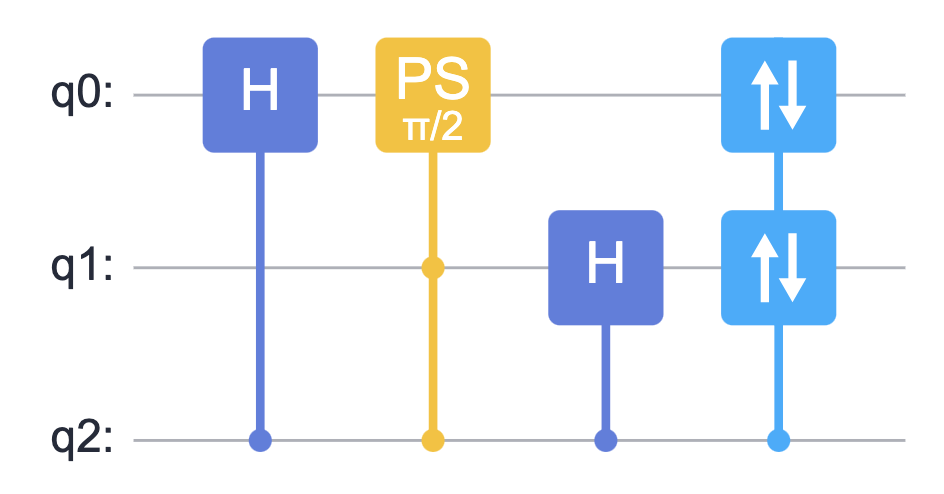
\includegraphics[width=0.9\linewidth]{2.3_figures/control.png}
    \caption{Add control qubits}
    \label{fig:controlled-method}
\end{figure}

In addition, we can add control bits to quantum circuits in batches. In the following example, the target qubits are q0 and q1, with control qubits q2 and q3, respectively:
\begin{lstlisting}
u = controlled(qft)
u = u([2, 3], [0, 1])
u.svg()
\end{lstlisting}

The result is shown in Fig.~\ref{fig:batch-control}.
\begin{figure}[h]
    \centering
    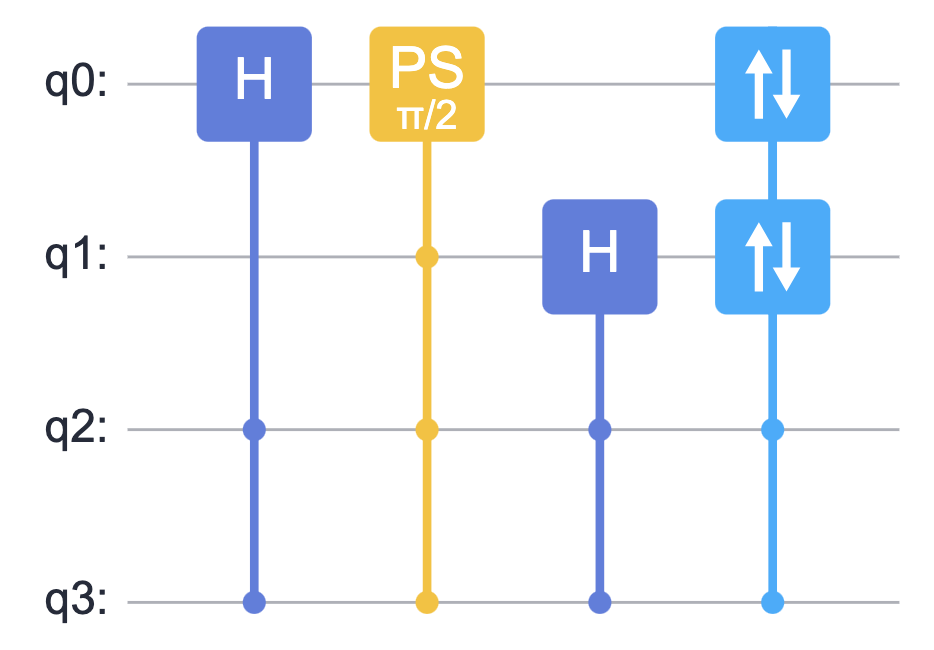
\includegraphics[width=0.9\linewidth]{2.3_figures/batch_control.png}
    \caption{Add control qubits in batches}
    \label{fig:batch-control}
\end{figure}

